
%(BEGIN_QUESTION)
% Copyright 2006, Tony R. Kuphaldt, released under the Creative Commons Attribution License (v 1.0)
% This means you may do almost anything with this work of mine, so long as you give me proper credit

Skisser kvalitativt hvordan en regulator med kun proporsjonalvirkning responderer over tid på følgende endringer i prosessvariabelen:

$$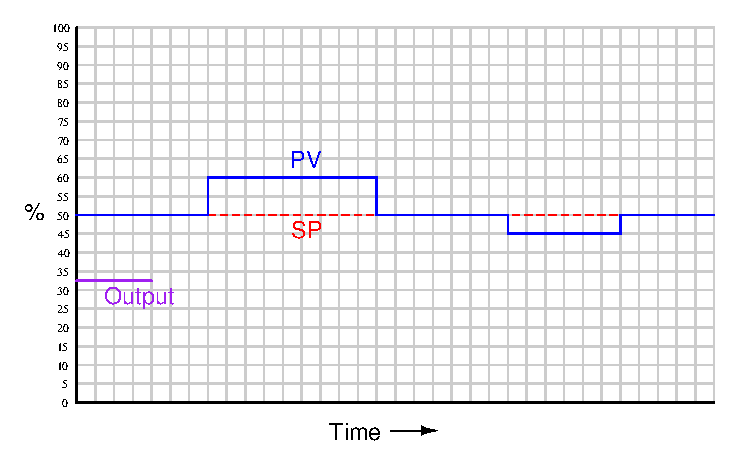
\includegraphics[width=15.5cm]{i01593x01.eps}$$

Anta {\it revers} reguleringsvirkning.

\vskip 20pt \vbox{\hrule \hbox{\strut \vrule{} {\bf Forslag til sokratisk diskusjon} \vrule} \hrule}

\begin{itemize}
\item{} Hva kjennetegner en ``reversvirkende'' regulator, i motsetning til en ``direktevirkende'' regulator?
\item{} Forklar hvorfor det ville være svært uvanlig å se en trend som dette i en reell, fungerende prosess-sløyfe. Hvorfor er denne trenden urealistisk, gitt en fungerende prosess der alle komponenter virker som de skal?
\item{} Gitt at trenden er urealistisk: hvorfor studerer vi den likevel? Med andre ord, hvilken verdi har en slik ``øvings-trend'' for oss?
\end{itemize}

\underbar{file i01593}
%(END_QUESTION)





%(BEGIN_ANSWER)

Regulatorutgangens graf vist her er kun {\it kvalitativ}. Selv om den er tegnet i riktig proporsjon (dvs. alle endringer i utgangen er riktig skalert relativt til hverandre), er selve skalaen vilkårlig og matcher derfor ikke nødvendigvis skalaen i din egen skisse:

$$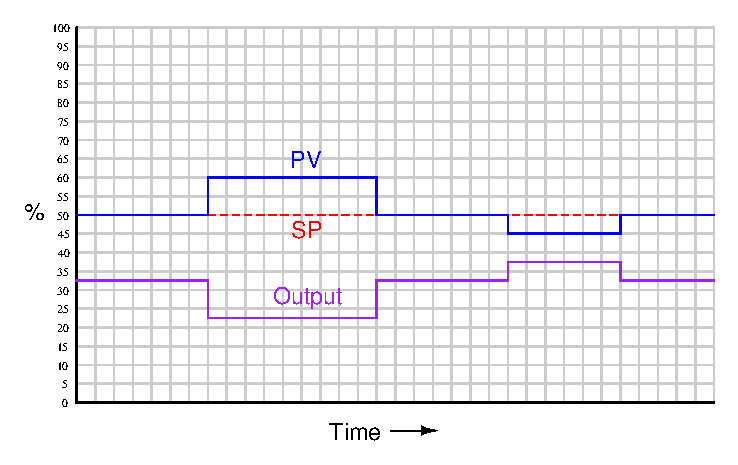
\includegraphics[width=15.5cm]{i01593x02.eps}$$

%(END_ANSWER)





%(BEGIN_NOTES)

Revers reguleringsvirkning betyr at utgangssignalet beveger seg motsatt vei av prosessvariabelen. Grafen er tegnet for en regulator med kun proporsjonalvirkning, med proporsjonalbånd på 100\% (forsterkning lik 1).

\vskip 10pt

{\bf Proporsjonalvirkning er når avvikets størrelse forteller utgangen hvor \underbar{langt} den skal gå.}

\vskip 10pt

{\bf Integralvirkning er når avvikets størrelse forteller utgangen hvor \underbar{raskt} den skal gå.}

\vskip 10pt

{\bf Derivatvirkning er når \underbar{hastigheten} til avviket forteller utgangen hvor \underbar{langt} den skal gå.}

%INDEX% Control, proportional: graphing controller response

%(END_NOTES)
